% Overview:
%   FastGT TeX subfile for the project.
%   Each subfile MUST start with the following line
%		\documentclass[../main.tex]{subfiles}

\documentclass[../main.tex]{subfiles}

\begin{document}

\subsection{FastGT}
\label{fastgt}

FastGT \cite{pajuste2017fastgt} è un metodo computazionale che conta le frequenze di k-mer unici nei dati delle read del genoma e utilizza queste informazioni per inferire i genotipi di varianti conosciute. FastGT è un tool molto veloce, in grado di rilevare le varianti in un genoma con coverage 30x\footnote{\ La \textit{coverage} è definita come il numero di basi di tutte le read brevi che corrispondono a un genoma diviso per la lunghezza di questo genoma.} in meno di 1 ora utilizzando un normale hardware a basso costo. Questo metodo fornisce un database di k-mer che può poi essere utilizzato per la genotipizzazione simultanea di circa trenta milioni di SNV (Single-Nucleotide Variant), inclusi più di 23.000 SNV dal cromosoma Y. Attualmente FastGT utilizza solo regioni affidabili del genoma ed è limitato alla chiamata di varianti genomiche note perché specifici k-mer devono essere preselezionati per tutti gli alleli noti; è ideale per una rapida analisi preliminare di un sottoinsieme di marcatori, successivamente seguita dall'analisi completa, quindi non sostituisce la mappatura tradizionale e la chiamata di varianti ma è un metodo complementare che facilita alcuni aspetti delle analisi del genoma.

Il metodo si basa su tre componenti: (1) la procedura per la selezione di k-mer unici, (2) la struttura dati personalizzata per l'archiviazione e il conteggio dei k-mer direttamente da un file FASTQ\footnote{\ FastQ è un formato di puro testo in codice ASCII facilmente leggibile, pensato dal Wellcome Sanger Institute per associare ad una sequenza prodotta da una tecnologia NGS, la qualità di ogni sua singola base. È diventato lo standard de facto per la condivisione di dati \cite{cock2010sanger} \label{nota:FASTQ}) prodotti da processi di sequenziamento basati su tecnologia NGS.} (vedi sezione \ref{AdaptiveRadixTree}) e (3) un metodo basato sulla probabilità progettato per stimare i genotipi dai conteggi dei k-mer.

\subsubsection{Adaptive radix tree}
\label{AdaptiveRadixTree}

L' Adaptive Radix Tree (ART) è una struttura dati progettata in \cite{leis2013art}. L'ART è basato sul \textit{trie} ma ottiene elevate prestazioni e efficienza in spazio, comprimendo l'albero sia verticalmente, ovvero, se un nodo non ha fratelli, viene unito con il suo genitore, riducendo l'altezza, e orizzontalmente, cioè utilizza un array che cresce con l'aumentare del numero di figli, riducendo le dimensioni di un nodo.

Ricordiamo che un \textit{trie} è una struttura dati ad albero ordinato usata per rappresentare un set, le cui chiavi sono tipicamente stringhe ordinate in ordine lessicografico; i nodi non conservano una copia della propria chiave, che dipende invece dalla posizione del nodo nell'albero. La radice è associata alla stringa vuota e tutti i discendenti di un nodo condividono il prefisso associato a quel nodo: attraversando l'albero si scende identificando la chiave parziale dei nodi. Le chiavi sono divise in chiavi parziali di s bit ciascuna, dove s è chiamato span: i nodi interni hanno 2s puntatori figlio (possibilmente nulli), uno per ogni possibile sequenza s-bit. Il vantaggio principale dei \textit{trie} rispetto all'hashing è l'ordinamento intrinseco. 

Ora vediamo come questa struttura viene migliorata, \textit{adattandola}. Quando si memorizzano chiavi lunghe, si formano catene di nodi in cui ogni nodo ha un solo figlio sprecando spazio perciò si può comprimere verticalmente e unire al padre ciascun nodo senza fratelli. Questo si può fare o nel modo pessimistico ``pessimistico", memorizzando una variabile aggiuntiva, chiamata prefisso, all'interno di ciascun nodo, che memorizza la concatenazione di chiavi parziali di discendenti che sono state eliminate perché non avevano fratelli, o in modo ``ottimista" memorizzando solo il numero di nodi compressi e nei nodi foglia le chiavi complete o in maniera ibrida, memorizzando il numero di nodi compressi e un array statico di dimensioni fisse per il percorso compresso.

Con grandi valori di span, si usa molto spazio con un'altezza ridotta: con nodi grandi viene allocato spazio per i puntatori ai nodi figlio, anche se non utilizzati. \cite{leis2013art} per effettuare la compressione orizzontale usa gli Adaptive Nodes, che utilizzano strutture dati dinamiche per tener conto dei figli, allocando meno spazio quando il numero di figli è piccolo e aggiungendone se vengono aggiunti più figli. Un nodo, a seconda del numero di nodi figlio, si trova quindi in una tra quattro configurazioni, ottimizzate per un diverso numero di figli. Quando le chiavi vengono inserite o eliminate i nodi vengono adattati di conseguenza (ad esempio la configurazione più compatta, \texttt{Nodo4}, può avere fino a quattro figli). Tutti i nodi hanno un'intestazione che memorizza il tipo di nodo, il numero di figli e la variabile prefisso, che contiene il percorso compresso (vedi \cite{leis2013art} per maggiori dettagli sulla struttura delle configurazioni). Vengono utilizzate poi \textit{single-value leaves}, ovvero i valori vengono memorizzati con un tipo di nodo foglia aggiuntivo che memorizza un valore.

Si possono effettuare operazioni di ricerca, che controlla la presenza di un elemento confrontando le chiavi e scendendo nell'albero, eliminazione, nella quale il nodo foglia identificato dalla chiave di ricerca viene rimosso da un nodo interno, controllando poi se necessario applicare la compressione verticale, ed inserzione.

Il layout variabile degli \textit{adaptive radix tree} consente di ottimizzare il database per diversi tipi di ricerche. Sia \textit{k} la lunghezza dei \textit{k}-mer che poi verranno inseriti nell'albero da FastGT, nel caso peggiore sia le ricerche che le inserzioni sono \textit{O}(log \textit{k}).



\subsubsection{Struttura Dati di FastGT}
\label{strutturaDatiFastGT}

L'input di FastGT è costituito da file FASTQ contenente i dati del genoma e da un database precompilato di varianti genomiche e corrispondenti coppie di k-mer che si sovrappongono a ciascuna variante. Ogni posizione bi-allelica del SNV nel genoma è coperta da k coppie di k-mer, dove la coppia è formata da k-mer corrispondenti a due alleli alternati: si presuppone che almeno un numero di queste siano uniche e appaiano esclusivamente in una posizione del genoma; pertanto, i conteggi di occorrenze di queste coppie di k-mer uniche nei dati di sequenziamento possono essere utilizzati per identificare il genotipo di questa variante in un individuo specifico. Sebbene una coppia di k-mer sia teoricamente sufficiente per la genotipizzazione, le mutazioni occasionalmente cambiano la sequenza del genoma nelle vicinanze di un SNV, impedendo il rilevamento del SNV, rischiando di far dedurre il genotipo sbagliato: si utilizzano quindi fino a tre coppie di k-mer per variante per prevenire chiamate errate causate da perdite occasionali di k-mer a causa di rare mutazioni. FastGT utilizza una lunghezza k = 25 dei k-mer. \\

\noindent
FastGT utilizza un adaptive radix tree (vedi Sezione \ref{AdaptiveRadixTree}) per memorizzare i k-mer e i relativi conteggi. Questa struttura dati permette di memorizzare  solo per i k-mer di interesse e le loro frequenze, anziché tutti i possibili k-mer del genoma. Inoltre permette un buon compromesso tra il consumo di memoria e la velocità di ricerca. 

I k-mer sono codificati con 2 bit per nucleotide e memorizzati come stringhe di bit. I rami possono dividere la stringa sia tra diversi nucleotidi sia all'interno di un nucleotide. Il \textit{trie} è composto da numeri interi a 64 bit, ciascuno interpretato o come parte unica più a destra di un k-mer (foglia) o come puntatore al ramo secondario successivo. L'albero non ha rami nel senso stretto del termine, ma i primi bit sono usati per selezionare il sottoalbero successivo. Le foglie sono interi a 64 bit. Anche i nodi dei rami sono codificati come singoli interi a 64 bit che contengono il valore, più un intero in più per ognuno dei rami successivi. Le stringhe di bit vengono memorizzate nel modo più compatto possibile, con delle parte di esse che possono essere interpretate come indice di un arco e altre parti come valori. (\textcolor{red}{prova a dirmi se si capisce perchè non so proprio come scriverlo, oppure tolgo e lascio più sottointeso.. volevo anche togliere la figura, ma è quella che fa capire.})
La Figura seguente \ref{fig:art} è un esempio di codifica di un 20-mer.

\begin{figure}[h!]
	\centering
  	\captionsetup{justification=centering}
  	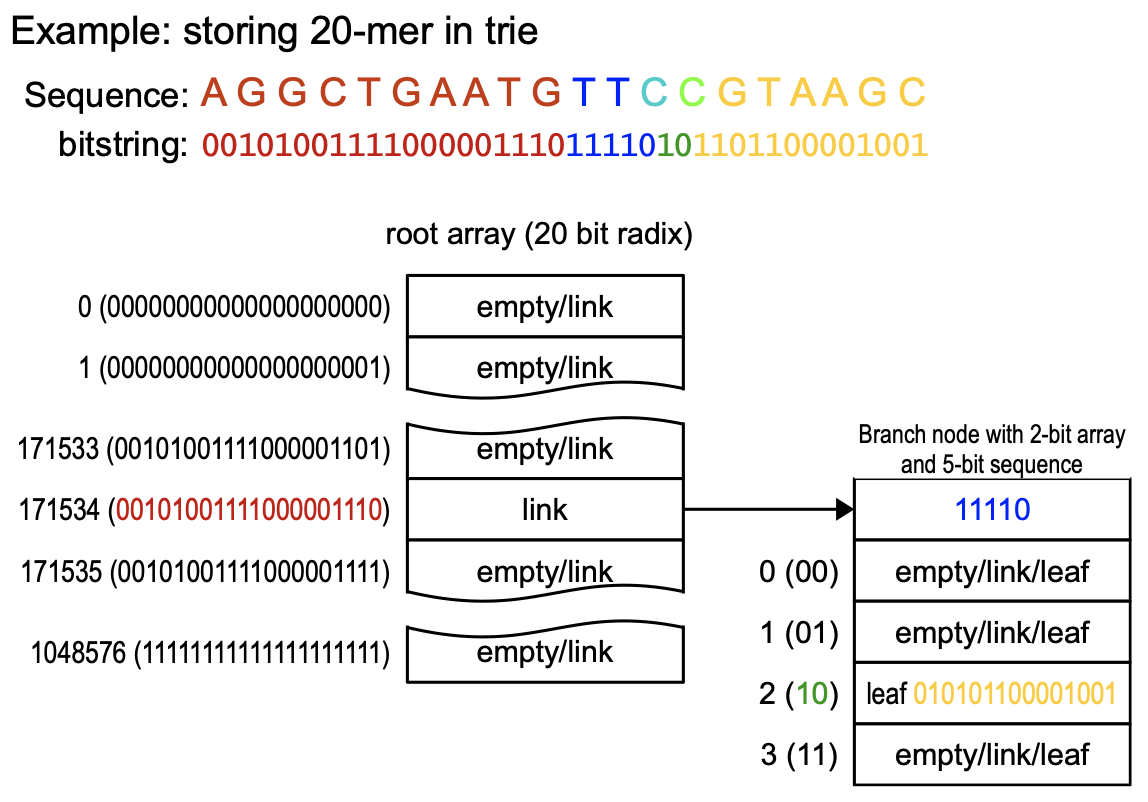
\includegraphics[scale=.35]{images/fastgt-art.png}
  	\caption{Layout semplificato dell'albero che memorizza 20-mer (40 bit), FastGT.}
  	\label{fig:art}
\end{figure}


\subsubsection{Algoritmo di FastGT}

Nella figura seguente è riportata la pipeline dell'algoritmo di FastGT (Figura \ref{fig:fastgt})

 \begin{figure}[h!]
	\centering
  	\captionsetup{justification=centering}
  	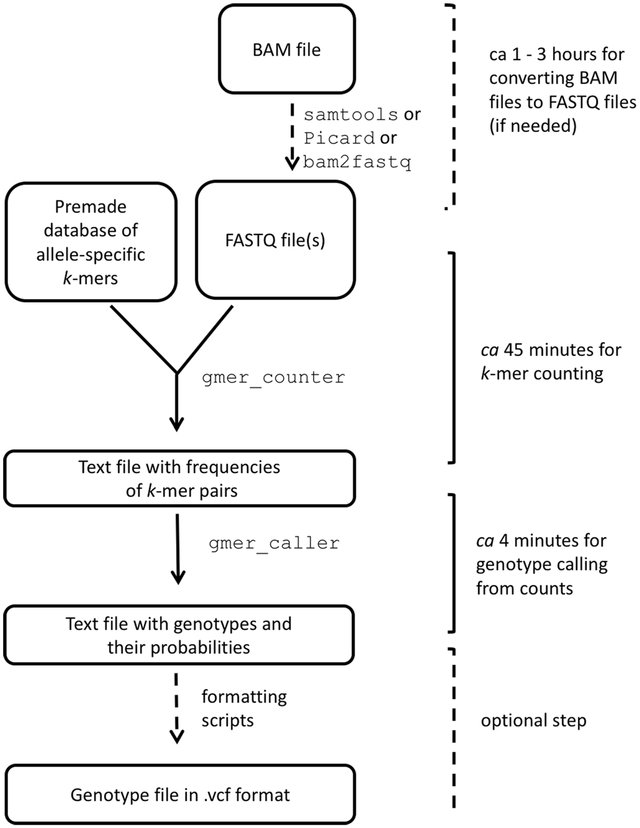
\includegraphics[scale=.25]{images/fastgt-pipeline.jpg}
  	\caption{Pipeline, FastGT.}
  	\label{fig:fastgt}
\end{figure}

\noindent
Il database delle varianti dei k-mer univoci viene assemblato identificando tutte le possibili coppie di k-mer per ogni variante, che poi vengono sottoposti a diversi passaggi di filtraggio. Le fasi di filtraggio rimuovono varianti per le quali non vengono osservati k-mer unici e varianti che producono genotipi non canonici (non diploidi negli autosomi e non aploidi nei cromosomi X e Y maschili) in una serie di test sequenziati da individui. La procedura di filtraggio è la seguente: partendo dagli SNV validati e gli indel comuni del database dbSNP (gli indel vengono usati solo per testare l'unicità dei k-mer, non vengono inclusi nel database delle varianti), per ogni SNV bi-allelico vengono create due sequenze attorno alla posizione dell'SNV: la sequenza del genoma di riferimento e quella corrispondente all'allele alternato. I k-mer vengono filtrati e vengono eliminati i k-mer che coprono un determinato SNV e che contengono altri SNV o indel noti, per rimuovere ogni possibile sovrapposizione: si vuole evitare di complicare gli algoritmi che effettuano il conteggio che dovrebbero tener conto di molteplici combinazioni di alleli SNV vicini. 

Nella seconda fase di filtraggio si testa l'unicità; il parametro di unicità è testato rispetto al genoma di riferimento espanso, l'insieme dei 25-mer dal genoma di riferimento più tutti i possibili 25-mer contenenti gli alleli alternati. Una coppia di k-mer è considerata unica se entrambi i k-mer si verificano non più di una volta nel genoma di riferimento espanso: tutte le coppie non uniche vengono rimosse.

Nella terza fase, i k-mer sono stati perfezionati testandone le frequenze, utilizzando le frequenze dei k-mer e i genotipi in un set di genomi di 50 individui sequenziati \footnote{\ Il DNA dei 50 individui casuali utilizzati è stato raccolto e sequenziato durante il Center of Translational Genomics project presso l'Università di Tartu; vengono usati 25 uomini e 25 donne per filtrare gli SNV autosomici, 50 uomini per chrX e chrY. }. Vengono rimosse le coppie di k-mer SNV con una frequenza anormalmente alta o un genotipo non canonico in più di un individuo.

Dopo le fasi di filtraggio, nel test riportato in \cite{pajuste2017fastgt} dal database dbSNP sono rimasti utilizzabili 30 238 283 (64\%) SNV bi-allelici validati. Inoltre è stato usato un sottoinsieme di marcatori SNV autosomici presenti sul microarray Illumina HumanOmniExpress per un'analisi di concordanza.  \\

\noindent
La genotipizzazione viene eseguita leggendo le read non elaborate e contandone le frequenze delle coppie di k-mer utilizzando il database precompilato delle varianti: si utilizza il software personalizzato \texttt{gmer\_counter} e \texttt{gmer\_caller}. Le frequenze di k-mer sono contate da \texttt{gmer\_counter}: si utilizza la struttura binaria degli adaptive radix tree (come citato precedentemente) per memorizzare sia le sequenze di k-mer che le loro frequenze. Le frequenze di un massimo di tre coppie di k-mer ottenute da \texttt{gmer\_counter} vengono salvate in un file di testo; infatti, per ridurre l'uso di k-mer ridondanti, tra le coppie di k-mer che si sovrappongono al SNV ne sono selezionate tre: si preferisce la coppia più a sinistra, la coppia più a destra e la coppia nel mezzo della regione, e se ciò non è possibile, perché una coppia non è univoca o contiene altri SNV, viene utilizzata la coppia k-mer più lontana successiva. In questo modo se una rara mutazione su un lato dell'SNV cambia la sequenza su quel lato, ci si aspetta che la coppia dall'altro lato abbia ancora i conteggi previsti. Le frequenze di tutte e tre le coppie siano conteggiate da \texttt{gmer\_counter} ma successivamente \texttt{gmer\_caller} utilizza solo la coppia con un conteggio di frequenza totale più vicino alla frequenza media in un dato individuo. Il file di testo in output viene utilizzato da \texttt{gmer\_caller} che determina i genotipi in base alle frequenze e stampa i risultati su un altro file di testo. 

\texttt{gmer\_caller} utilizza la regola Bayes (come gli altri tool precedentemente analizzati) per chiamare i genotipi, a partire dalle frequenze dei k-mer, assegnando a ciascuna variabile il genotipo più probabile. Le distribuzioni di frequenza degli alleli (di riferimento e alternativi) sono modellate da una distribuzione binomiale negativa con media uguale al prodotto della coverage e la vera molteplicità del k-mer nel genoma; il modello consente di stimare il numero di copie più probabile per entrambi gli alleli. Dati i conteggi degli alleli osservati, \texttt{gmer\_caller} calcola la probabilità di ciascun genotipo applicando la regola di Bayes e restituisce come genotipo chiamato, quello con la maggiore probabilità. 

Il genere dell'individuo viene determinato automaticamente dai dati di sequenziamento utilizzando, la frequenza media dei marker dal cromosoma X (chrX): se l'individuo è femmina, nel processo di chiamata viene utilizzato solo il modello autosomico (per chiamare gli SNV sia negli autosomi che nel cromosoma X) e non vengono chiamati i marcatori del cromosoma Y (chrY), per gli uomini un ulteriore modello aploide del classificatore di Bayes è addestrato per chiamare i genotipi degli SNV negli autosomi e anche nei cromosomi sessuali.


\subsubsection{Prestazioni di FastGT}

Al fine di testare le prestazioni di FastGT, \cite{pajuste2017fastgt} eseguono numerosi test\footnote{\ Le prestazioni sono state testate su un server Linux con 32 core CPU, 512 GB di RAM e IBM 6 Gbps and SAS 7200 rpm disk drives in una configurazione RAID10 \cite{pajuste2017fastgt}.}. Durante l'esposizione dei risultati si assumerà come A l'allele di riferimento e B l'allele alternato.

Per quanto riguarda la quantità minima di memoria richiesta dall'algoritmo, essa è determinata dalla dimensione della struttura dati usata da \texttt{gmer\_counter} (vedi Sezione \ref{strutturaDatiFastGT}). Rispetto al tempo, l'algoritmo è molto veloce (circa 40 minuti su un server con 32 Core di CPU per identificare i 30 milioni di SNV dai dati di sequenziamento di un singolo individuo (\textit{coverage} 30x) la maggior parte è dedicata al conteggio delle frequenze mentre la chiamata del genotipo con \texttt{gmer\_caller} richiede circa 2-3 minuti con 16 Core. (\textcolor{red}{*})

In \cite{pajuste2017fastgt}, inizialmente vengono generate delle read grezze simulate dal genoma di riferimento per analizzare la capacità del classificatore bayesiano di chiamare i genotipi del genoma di riferimento (assunto come omozigote in tutte le posizioni (indicato come AA)); in questa simulazione la frazione del genotipo corretto recuperato variava tra il 98,94\% (con \textit{coverage} 5x) e il 99,95\% (con \textit{coverage} 20x). La frazione di marcatori non chiamati era compresa tra 0,001\% (con \textit{coverage} 20x) e 1,036\% (con \textit{coverage} 5x). La frazione delle chiamate AB era compresa tra lo 0,02\% e lo 0,05\%.
 
Per stimare le prestazioni delle chiamate dei genotipi AB e BB vengono creati genomi simulati utilizzando genotipi da 5 individui di diverse popolazioni. Si riscontra che la sensibilità, la frazione di chiamate corrette AB e BB è fortemente influenzata dalla copertura (61\% con \textit{coverage} 5x, 99,8\% con \textit{coverage} 20x), ma non è condizionata dalle diverse popolazioni degli individui. di diverse popolazioni: 99,7–99,8\% con copertura 30x (Fig. 3). La specificità, frazione di chiamate AA corrette, rimane uniformemente alta tra il 99,60\% e il 99,95\%. Questi risultati mostrano che il dataset di 30 milioni di marcatori è utilizzabile per studiare popolazioni diverse senza distorsioni di sensibilità o specificità.

Per quanto riguarda l'accuratezza delle chiamate, essa è stata analizzata confrontando i risultati con i genotipi riportati in due individui del dataset Illumina Platinum (\textit{coverage} 50x). La concordanza complessiva dei genotipi bi-allelici predetti da FastGT rispetto ai due genomi è del 99,96\%. La concordanza delle chiamate con alleli non di riferimento (AB o BB) è stata del 99,93\% mentre non è stato chiamato solo lo 0,24\%. (\textcolor{red}{secondo te la metto una tabella per questo? cioè io la vorrei anche mettere ma viene troppo.. pensavo di togliere questi numeri ma alla fine in FastGT non ci sono confronti con altri tool, quindi un minimo di prestazioni volevo metterle, alla fine queste sono prestazioni di accuratezza, non tempo e memoria, forse tolgo la parte su tempo e memoria dove ho messo *... ti chiedo anche una tua opinione})

Viene analizzato successivamente in che modo la \textit{coverage} del sequenziamento del genoma influisce sulle prestazioni di FastGT; nella maggior parte degli scenari è preferibile una \textit{coverage} non eccessivamente elevata per ottimizza i costi. Sono stati costruiti dei set con \textit{coverage} diverse e viene esaminata l'accuratezza: si osserva che in generale la concordanza con i genomi del dataset Illumina Platinum sono corrette, soprattutto per quanto riguarda la chiamata di genotipi di riferimento; per quanto riguarda i genotipi non di riferimento (AB e BB) la concordanza diminuisce significativamente quando la copertura scende al di sotto di 20x. L'uniformità della \textit{coverage} e la frazione di errori di sequenziamento sono comunque i principali fattori che influenzano il conteggio dei k-mer, perché un tasso di errore più elevato riduce il numero di k-mer utilizzabili e introduce rumore indesiderato. 

Infine, è opportuno riportare un'analisi sulla lunghezza dei k-mer utilizzata: FastGT imposta k = 25, anche se FastGT è in grado di usare anche altre lunghezze tra 16 e 32. Se si utilizzano k-mer più corti di 20 nucleotidi un numero piuttosto elevato di marcatori viene eliminato dal set nelle fasi di filtraggio, ma questo numero non aumenta in modo significativo per k maggiore di 24. Non viene confrontata l'accuratezza con diverse lunghezze dei k-mer, ma ci si aspetta che questi due fattori siano relativamente indipendente. \\

\noindent
FastGT non ha attualmente alcuna capacità di chiamare varianti \textit{de novo} ed è limitato alla chiamata di sottoinsiemi di varianti predefinite; esso non si limita all'identificazione di SNV, qualsiasi variante nota che può essere associata a un k-mer unico e specifico per variante può essere rilevata con FastGT, come ad esempio indel corti ma non per varianti strutturali. Inoltre FastGT è stato utilizzato solo con i dati di sequenziamento Illumina, ma in linea di principio è utilizzabile con altre tecnologie di sequenziamento.


\end{document}